
\chapter{Caracterização do Protótipo}
\label{cha:prototipo}

Neste capítulo, é detalhada a abordagem utilizada para a realização do projeto.

\section{Protótipo}

O projeto foi desenvolvido seguindo uma abordagem de prototipagem evolutiva, ilustrada na \figurename~\ref{fig:proto}. Com a implementação do protótipo, foi possível reduzir as incertezas em torno do projeto.

\begin{figure}[ht]
	\centering
	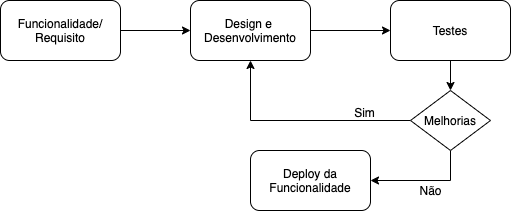
\includegraphics[width=0.85\textwidth]{proto}
	  \caption{Protótipo evolutivo}
  \label{fig:proto}
\end{figure}

\textbf{Funcionalidade/Requisito}, é realizado o levantamento das necessidades da funcionalidade a ser implementada e se é viável para o sistema. Após o levantamento, é realizado o \textbf{Design e Desenvolvimento} da funcionalidade, de ponta a ponta, sendo realizados \textbf{Testes/Análises} para detetar possíveis problemas e se de facto é o ideal para o objetivo do trabalho. Com a conclusão dos testes, o processo de design e desenvolvimento pode ser repetido/revisto de forma a melhorar a funcionalidade. Caso não seja necessário melhorias, é realizado o \textbf{Deploy da funcionalidade}, dando assim como concluída. 

\section{Tecnologias e frameworks utilizadas}

Antes do início da implementação do projeto, foi importante a escolha das tecnologias e \textit{frameworks} corretas de forma a fornecer aos utilizadores do sistema as funcionalidades desejadas, garantindo a interoperabilidade entre todas as componentes do sistema.   

As tecnologias utilizadas foram escolhidas maioritariamente pelo facto de já ter conhecimento e ter trabalhado com elas, tanto a nível profissional como académico, o que permitiu focar os esforços nos aspetos/requisitos do projeto.

\textbf{Spring Boot} \cite{spring} (utilizando a linguagem \textit{kotlin}) foi a \textit{framework} escolhida para criar a componente servidor do sistema, pela facilidade que oferece na configuração \textit{Spring}, permitindo o rápido desenvolvimento de aplicações. 

\textbf{Android} (utilizando a linguagem \textit{kotlin}), foi escolhido para fornecer ao utilizador a aplicação cliente do sistema, por ser a tecnologia mais utilizada em dispositivos móveis e a que tenho maiores valências por ser a área de maior foco a nível profissional. 	

\textbf{Flutter Web} \cite{flutter} com a linguagem \textit{dart}, é a opção para o simulador de serviço, que tem como objetivo simular aquilo que acontece em postos de serviços, em relação ao avanço das filas, permitindo também a configuração (criação, atualização e eliminação) dos serviços, dos postos e das filas. Por ter já experiência em desenvolvimento de aplicação móveis a nível profissional utilizando o \textit{flutter}, o simulador surgiu como oportunidade para desenvolver as minhas capacidades mais direcionadas para a Web, levando à escolha da \textit{framework}. 

\textbf{\acrfull{fcm}} \cite{firebase} é a solução escolhida para realizar a entrega de mensagem/notificações aos utilizadores por parte do servidor o que permite realizar a atualização em tempo do estado das filas de espera. Escolhida pelo facto de ser uma solução confiável e sem custos, sendo a única dependência externa do sistema.  

\textbf{Heroku} \cite{heroku} foi a plataforma em nuvem escolhida para realizar o \textit{deploy} do servidor e do simulador de serviço, visto ser uma plataforma que suporta várias linguagens, permitindo a hospedagem desde protótipos (sem custo) a aplicações empresariais. 

\textbf{Node.JS} \cite{nodejs} é utilizado simplesmente para a criação de um servidor que permite exibir/expor o Javascript/HTML/CSS estático gerado através do \textit{flutter web}. Foi desenvolvido esta solução pelo facto do Heroku não ter ainda a capacidade de construir aplicações em \textit{flutter web}, nem de exibir ficheiros estáticos visto que o objetivo da plataforma é mais focada em servir requisitos a nível do servidor. 

\section{Requisitos}

Para a realização deste projeto, foi feito o levantamento dos requisitos funcionais e não funcionais gerais do sistema, que foram incrementando à medida que o protótipo foi avançando, identificando em primeiro lugar os atores do sistema. A especificação dos requisitos está estruturada sob a forma de modelo de casos de utilização.

\subsection{Ambiente/Contexto de utilização}

O contexto de utilização, presente na \figurename~\ref{fig:contextoutilizacao} é a representação geral do sistema, onde os atores dão inicio a operações/ações (casos de utilização), obtendo e visualizando resultados devolvidos pelo sistema. 

\begin{figure}[ht]
	\centering
	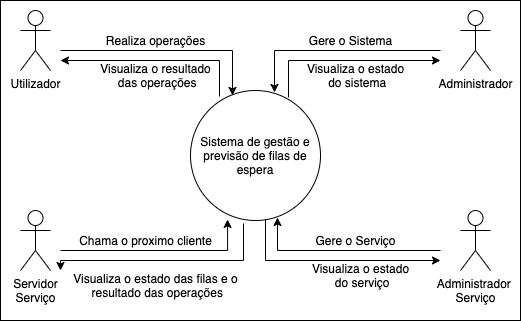
\includegraphics[width=0.85\textwidth]{contextoutilizacao}
	\caption{Contexto de Utilização}
  	\label{fig:contextoutilizacao}
\end{figure}

Conceitos apresentados na \figurename~\ref{fig:contextoutilizacao}: 

\begin{itemize}
	\item Atores/Entidades (utilizador, administrador, servidor de serviço e administrador de serviço) - entidade externa que interage com o sistema de forma a realizar trabalho, mas sobre a qual não tem controlo, estando fora da influência do sistema.
	\item Sistema de gestão e previsão - Realiza um conjunto de operações de acordo com as ações dos atores.
	\item Fluxos/Interação - Comunicação entre os atores e o sistema.
\end{itemize}

\subsection{Diagramas de Casos de Utilização}

Os diagramas de caso de utilização especificam os comportamentos resultantes da interação entre atores e sistema para atingir um objetivo. Para cada tipo de ator identificado, nomeadamente servidor de serviço (\figurename~\ref{fig:casosutilizacaoserver}), utilizador (\figurename~\ref{fig:casosutilizacaouser}), administrador (\figurename~\ref{fig:casosutilizacaoadmin}) e administrador de serviço (\figurename~\ref{fig:casosutilizacaoserviceadmin}), é apresentado o respetivo diagrama. 

\begin{figure}[ht]
	\centering
	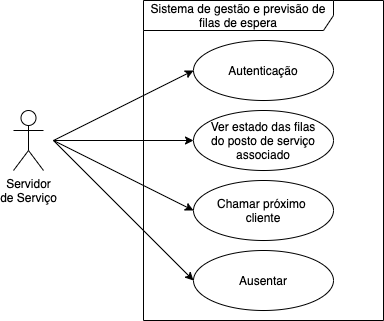
\includegraphics[width=0.85\textwidth]{casosutilizacaoserver}
	\caption{Casos de utilização do servidor de serviço}
  	\label{fig:casosutilizacaoserver}
\end{figure}

\begin{figure}[hp]
	\centering
	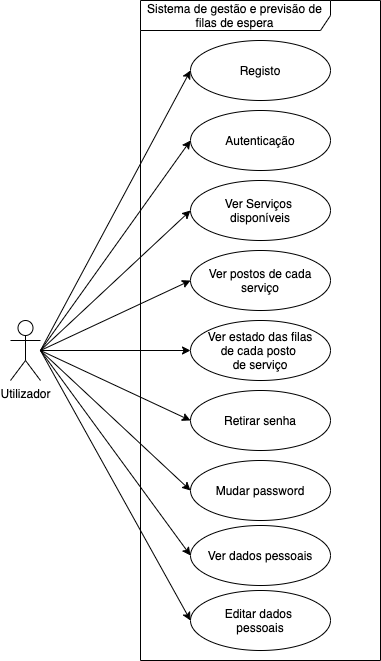
\includegraphics[width=0.85\textwidth,height=1\textwidth]{casosutilizacaouser}
	\caption{Casos de utilização do utilizador}
  	\label{fig:casosutilizacaouser}
\end{figure}

\begin{figure}[hp]
	\centering
	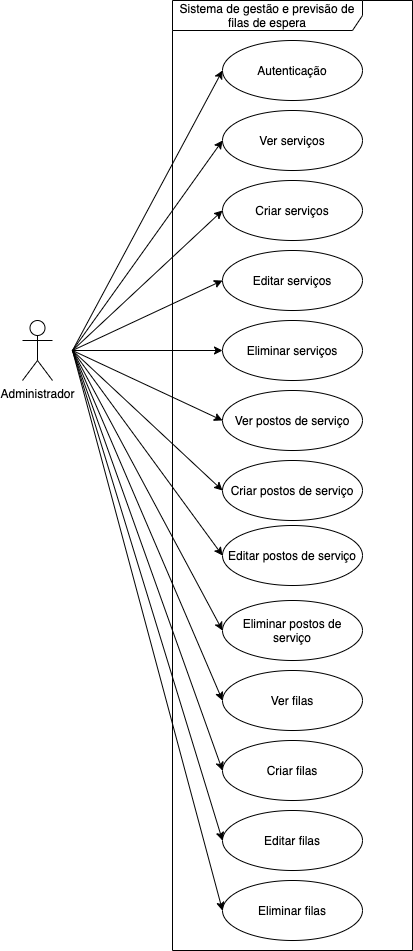
\includegraphics[scale=0.6]{casosutilizacaoadmin}
	\caption{Casos de utilização do administrador}
  	\label{fig:casosutilizacaoadmin}
\end{figure}

\begin{figure}[hp]
	\centering
	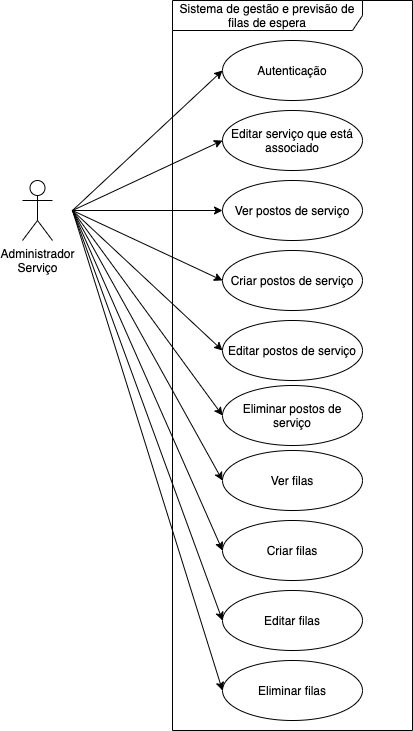
\includegraphics[scale=0.75]{casosutilizacaoserviceadmin}
	\caption{Casos de utilização do administrador de serviço}
  	\label{fig:casosutilizacaoserviceadmin}
\end{figure}

\newpage

\subsection{Descrição dos Casos de Utilização}

Cada caso de utilização descreve o que pode acontecer (operação) no sistema e apresentado ao utilizador quando este realiza uma determinada ação.

{\large \textbf{Registo do Utilizador}} \\
\textbf{Ator}: Utilizador \\
\textbf{Cenário Principal}:

\begin{enumerate}[nolistsep]
	\item O utilizador inicia a aplicação móvel
	\item A aplicação apresenta a janela de registo
	\item O utilizador preenche com os dados requisitados
	\item O sistema valida os dados. Se os dados forem válidos apresenta ao utilizador uma mensagem de sucesso
\end{enumerate}

\textbf{Cenário Alternativo A}:
\begin{enumerate}[nolistsep]
	\item No passo 4, os dados não são válidos
	\item O sistema apresenta ao utilizador os campos que não estão válidos
\end{enumerate}

{\large\textbf{Autenticação do Utilizador}} \\
\textbf{Ator}: Utilizador, Administrador, Servidor e Administrador de serviço \\
\textbf{Cenário Principal}:

\begin{enumerate}[nolistsep]
	\item O utilizador inicia a aplicação móvel ou web
	\item A aplicação apresenta a janela de autenticaçao
	\item O utilizador preenche com os dados de autenticação (\textit{username} e \textit{password})
	\item O sistema valida os dados. Se forem válidos apresenta uma página com os serviços disponíveis
\end{enumerate}

\textbf{Cenário Alternativo A}:
\begin{enumerate}[nolistsep]
	\item No passo 4, os dados não são válidos
	\item A aplicação apresenta uma mensagem ao utilizador informando que a autenticação não é válida
\end{enumerate}

{\large\textbf{Ver Serviços}} \\
\textbf{Ator}: Administrador e utilizador \\
\textbf{Cenário Principal}:

\begin{enumerate}[nolistsep]
	\item Incluir "Autenticação do Utilizador"
	\item O sistema apresenta os serviços disponíveis
\end{enumerate}

{\large\textbf{Criar Serviços}} \\
\textbf{Ator}: Administrador  \\
\textbf{Cenário Principal}:

\begin{enumerate}[nolistsep]
	\item Incluir "Ver Serviços"
	\item O utilizador seleciona a opção para criar serviços
	\item O sistema apresenta um formulário para criação de um serviço
	\item O utilizador preenche o formulário e submete.
	\item O sistema processa o novo serviço.
	\item O sistema apresenta os serviços disponíveis atualizado 
\end{enumerate}

{\large\textbf{Editar Serviços}} \\
\textbf{Ator}: Administrador e administrador de serviço  \\
\textbf{Cenário Principal - Administrador}:

\begin{enumerate}[nolistsep]
	\item Incluir "Ver Serviços"
	\item O utilizador seleciona o serviço que pretende editar
	\item O sistema apresenta um formulário com informação editável do serviço
	\item O utilizador edita o formulário e submete.
	\item O sistema processa a edição do serviço e apresenta mensagem de sucesso.
\end{enumerate}

\textbf{Cenário Principal - Administrador de serviço}:
\begin{enumerate}[nolistsep]
	\item Incluir "Autenticação do Utilizador"
	\item O sistema apresenta um formulário com informação editável do serviço
	\item O utilizador edita o formulário e submete.
	\item O sistema processa a edição do serviço e apresenta mensagem de sucesso.
\end{enumerate}

{\large\textbf{Eliminar Serviços}} \\
\textbf{Ator}: Administrador \\
\textbf{Cenário Principal}:

\begin{enumerate}[nolistsep]
	\item Incluir "Ver Serviços"
	\item O utilizador seleciona o serviço que pretende eliminar
	\item O utilizador requisita a eliminação do serviço e aprova.
	\item O sistema processa a eliminação e apresenta os serviços disponíveis atualizado.
\end{enumerate}

\textbf{Cenário Alternativo A}:

\begin{enumerate}[nolistsep]
	\item No passo 3, o utilizador rejeita.
	\item O sistema permanece no serviço selecionado.
\end{enumerate}

{\large\textbf{Ver Postos de Serviço}} \\
\textbf{Ator}: Administrador, administrador de serviço e utilizador \\
\textbf{Cenário Principal}:

\begin{enumerate}[nolistsep]
	\item Incluir "Ver Serviços" 
	\item O utilizador seleciona o serviço que pretende ver 
	\item O sistema apresenta a informação do serviço e os postos associados
\end{enumerate}

{\large\textbf{Criar Postos de Serviço}} \\
\textbf{Ator}: Administrador e administrador de serviço \\
\textbf{Cenário Principal}:

\begin{enumerate}[nolistsep]
	\item Incluir "Ver Postos de Serviço"
	\item O utilizador seleciona a opção para criar um posto
	\item O sistema apresenta um formulário 
	\item O utilizador preenche o formulário e submete.
	\item O sistema processa o novo posto.
	\item O sistema apresenta o serviço com os postos disponíveis atualizado 
\end{enumerate}

{\large\textbf{Editar Postos de Serviço}} \\
\textbf{Ator}: Administrador e administrador de serviço \\
\textbf{Cenário Principal}:

\begin{enumerate}[nolistsep]
	\item Incluir "Ver Postos de Serviço"
	\item O utilizador seleciona o posto pretendido
	\item O sistema apresenta um formulário editável do posto de serviço
	\item O utilizador edita o formulário e submete.
	\item O sistema processa a edição do serviço e apresenta mensagem de sucesso.
\end{enumerate}

{\large\textbf{Eliminar Postos de Serviço}} \\
\textbf{Ator}: Administrador e administrador de serviço \\
\textbf{Cenário Principal}:

\begin{enumerate}[nolistsep]
	\item Incluir "Ver Postos de Serviço"
	\item O utilizador seleciona o posto pretendido
	\item O sistema apresenta um formulário editável do posto de serviço
	\item O utilizador requisita a eliminação do posto e aprova.
	\item O sistema processa a eliminação e apresenta o serviço com os postos disponíveis atualizado.
\end{enumerate}

\textbf{Cenário Alternativo A}:

\begin{enumerate}[nolistsep]
	\item No passo 4, o utilizador rejeita.
	\item O sistema permanece no posto selecionado.
\end{enumerate}

{\large\textbf{Ver Filas}} \\
\textbf{Ator}: Administrador, utilizador, administrador e servidor de serviço\\
\textbf{Cenário Principal Administrador, Utilizador e Administrador de Serviço}:

\begin{enumerate}[nolistsep]
	\item Incluir "Ver Postos de Serviço" 
	\item O utilizador seleciona o posto de serviço que pretende ver 
	\item O sistema apresenta a informação do posto serviço e as filas associadas
\end{enumerate}

\textbf{Cenário Principal Servidor de Serviço}:

\begin{enumerate}[nolistsep]
	\item Incluir "Autenticação do Utilizador" 
	\item O sistema apresenta a informação do posto serviço associado ao utilizador e as filas associadas
\end{enumerate}

{\large\textbf{Criar Filas}} \\
\textbf{Ator}: Administrador e administrador de serviço \\
\textbf{Cenário Principal}:

\begin{enumerate}[nolistsep]
	\item Incluir "Ver Filas"
	\item O utilizador seleciona a opção para criar uma fila
	\item O sistema apresenta um formulário 
	\item O utilizador preenche o formulário e submete.
	\item O sistema processa a nova fila.
	\item O sistema apresenta o posto serviço com as filas disponíveis atualizado
\end{enumerate}

{\large\textbf{Editar Filas}} \\
\textbf{Ator}: Administrador e administrador de serviço \\
\textbf{Cenário Principal}:

\begin{enumerate}[nolistsep]
	\item Incluir "Ver Filas"
	\item O utilizador seleciona a fila pretendida
	\item O sistema apresenta um formulário editável da fila
	\item O utilizador edita o formulário e submete.
	\item O sistema processa a edição da fila e apresenta mensagem de sucesso.
\end{enumerate}

{\large\textbf{Eliminar Filas}} \\
\textbf{Ator}: Administrador e administrador de serviço \\
\textbf{Cenário Principal}:

\begin{enumerate}[nolistsep]
	\item Incluir "Ver Filas"
	\item O utilizador seleciona a fila pretendida
	\item O sistema apresenta um formulário editável da fila
	\item O utilizador requisita a eliminação da fila e aprova.
	\item O sistema processa a eliminação e apresenta o posto de serviço com as filas disponíveis atualizado.
\end{enumerate}

\textbf{Cenário Alternativo A}:

\begin{enumerate}[nolistsep]
	\item No passo 4, o utilizador rejeita.
	\item O sistema permanece na fila selecionada.
\end{enumerate}


{\large\textbf{Chamar próximo cliente}} \\
\textbf{Ator}: Servidor de serviço \\
\textbf{Cenário Principal}:

\begin{enumerate}[nolistsep]
	\item Incluir "Ver Filas"
	\item O utilizador realiza a ação chamar próximo cliente caso a tolerância já tenha passado.
	\item O sistema faz a chamada, alterando o estado da fila
\end{enumerate}

\textbf{Cenário Alternativo A}:

\begin{enumerate}[nolistsep]
	\item No passo 3, o sistema dá uma mensagem a indicar que ainda não pode chamar o próximo cliente
\end{enumerate}

{\large\textbf{Ausentar}} \\
\textbf{Ator}: Servidor de serviço \\
\textbf{Cenário Principal}:

\begin{enumerate}[nolistsep]
	\item Incluir "Autenticação do Utilizador"
	\item O utilizador realiza a ação para ausentar do posto de trabalho
\end{enumerate}

{\large\textbf{Regressar}} \\
\textbf{Ator}: Servidor de serviço \\
\textbf{Cenário Principal}:

\begin{enumerate}[nolistsep]
	\item Incluir "Autenticação do Utilizador"
	\item O utilizador realiza a ação para regressar ao posto de trabalho
\end{enumerate}

{\large\textbf{Retirar Senha}} \\
\textbf{Ator}: Utilizador \\
\textbf{Cenário Principal}:

\begin{enumerate}[nolistsep]
	\item Incluir "Ver Filas"
	\item O utilizador seleciona a fila pretendida
	\item O sistema apresenta a fila ao utilizador
	\item O utilizador realiza a ação de obtenção de senha
	\item O sistema processa o pedido, criando serviços para apresentar ao utilizador a atualização do estado das filas
\end{enumerate}

{\large\textbf{Ver dados pessoais}} \\
\textbf{Ator}: Utilizador \\
\textbf{Cenário Principal}:

\begin{enumerate}[nolistsep]
	\item Incluir "Autenticação do Utilizador"
	\item O utilizador seleciona o menu/definições
	\item O sistema apresenta os dados do utilizador
\end{enumerate}

{\large\textbf{Editar dados pessoais}} \\
\textbf{Ator}: Utilizador \\
\textbf{Cenário Principal}:

\begin{enumerate}[nolistsep]
	\item Incluir "Ver dados pessoais"
	\item O utilizador edita os dados editáveis e submete
	\item O sistema dá mensagem de sucesso
\end{enumerate}

{\large\textbf{Mudar Password}} \\ 
\textbf{Ator}: Utilizador \\
\textbf{Cenário Principal}:

\begin{enumerate}[nolistsep]
	\item Incluir "Incluir "Ver dados pessoais"
	\item O utilizador escolhe a opção para alterar a password
	\item O utilizador edita a password e submete
	\item O sistema dá mensagem de sucesso	
\end{enumerate}

\subsection{Diagrama de Sequência}

Na \figurename~\ref{fig:diagramasequencia}, é apresentado o diagrama de sequência na perspectiva do utilizador, que permite a entrada na aplicação para autenticação assim como a obtenção de uma senha num posto de serviço, conseguindo visualizar o tempo de espera previsto.

\begin{figure}[H]
	\centering
	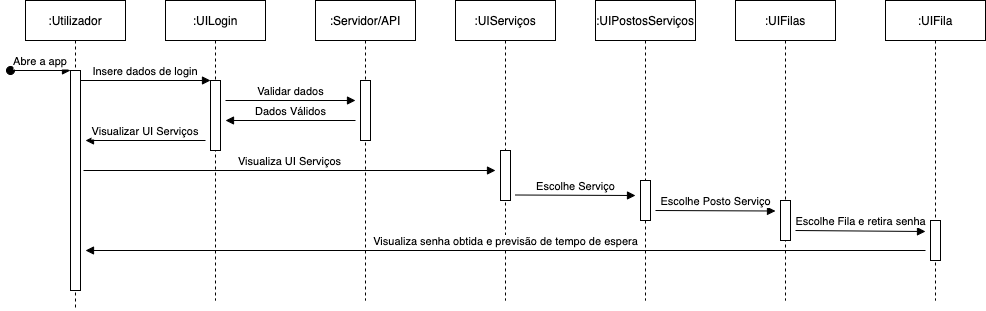
\includegraphics[width=1\textwidth]{diagramasequencia}
	  \caption{Diagrama de sequência}
  \label{fig:diagramasequencia}
\end{figure}

O utilizador ao abrir a aplicação móvel é lhe apresentado o ecrã de login, onde deve indicar as credenciais corretas de forma a realizar a autenticação no sistema. Ao realizar o pedido de autenticação, os dados são enviados ao servidor de forma a realizar a validação. Em caso de sucesso o utilizador é reencaminhado para o ecrã onde consegue ver os serviços disponíveis, caso contrário é apresentado uma mensagem indicando que as credenciais não estão corretas. O utilizador no ecrã dos serviços, tem a possibilidade de escolher o pretendido, sendo apresentado os postos que o serviço tem para os atendimentos. Em caso de escolha de um dos postos, é apresentado as filas com detalhes como tempo de espera previsto, nome/descrição da fila e o número que está a ser atendido. O utilizador pode escolher uma das filas e retirar uma senha, onde passa a receber atualizações em tempo real sobre o estado da fila.

\section{Modelo Domínio}

Na \figurename~\ref{fig:modelodominio}, é apresentado o modelo sobre a qual o sistema se baseia.

\begin{figure}[H]
	\centering
	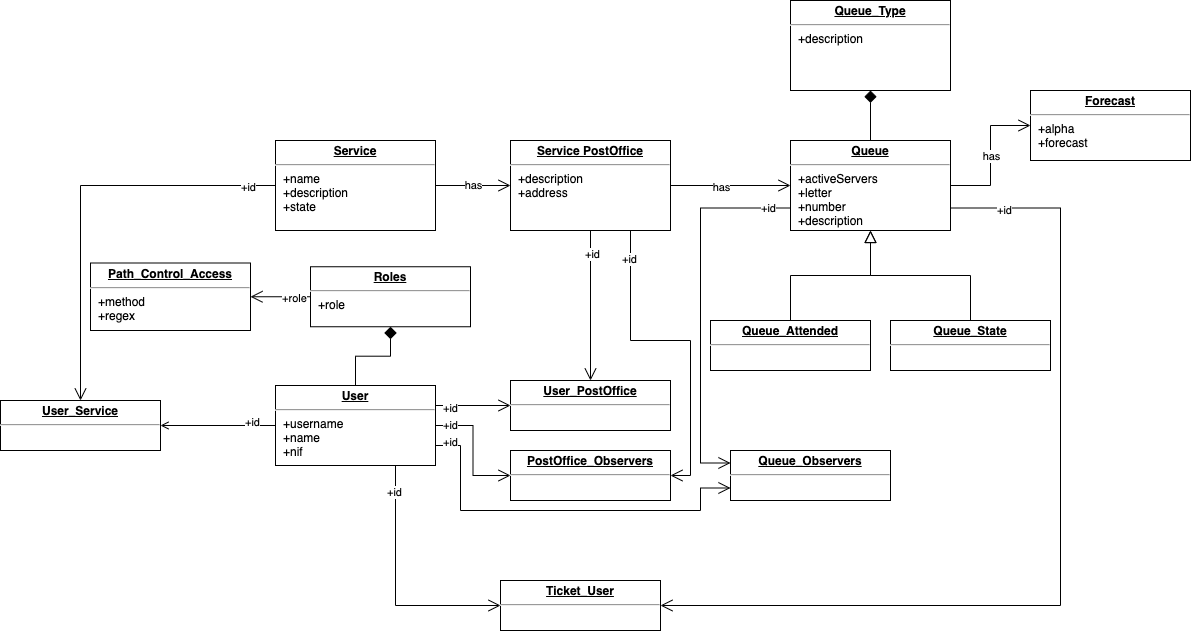
\includegraphics[width=1\textwidth]{modelodominio}
	  \caption{Modelo de Domínio}
  \label{fig:modelodominio}
\end{figure}

O modelo representado na \figurename~\ref{fig:modelodominio}, apresenta as entidades resultantes dos requisitos do projeto. Para simplificação, não é incluído todas as caracteristicas/propriedades das entidades. Cada entidade representa um tipo de informação do domínio do problema. A entidade \textbf{\textit{User}}, com os atributos, \textit{name}, \textit{username}, \textit{nif}, representa todos os utilizadores que fazem parte do sistema. Recorrendo à agregação com \textbf{\textit{Roles}} é possível diferenciar o papel que cada utilizador pode ter no sistema, conseguindo apenas realizar as operações autorizadas para cada papel de forma a garantir os comportamentos corretos. Com a entidade \textbf{\textit{Path\_Control\_Access}}, é possível definir as regras de acesso para cada tipo de utilizador. Com as entidades \textbf{\textit{User\_Service}} e \textbf{\textit{User\_PostOffice}}, um administrador poderá definir em que serviços e postos de serviços é que cada utilizador pode realizar operações sobre, desde que tenha o papel correto para o efeito. \textbf{\textit{Service}} representa os serviços institucionais, tendo cada serviço um conjunto de postos de serviço (\textbf{\textit{Service\_PostOffice}}), onde um utilizador pode realizar o tratamento dos assuntos de interesse. Para tratamento de assuntos em cada posto de serviço existe um conjunto de filas, representado pela entidade \textbf{\textit{Queue}} que podem ter propósitos diferentes e prioridades diferentes, representado por \textbf{\textit{Queue\_Type}}, o que permite ter regras apropriadas na gestão das senhas dos utilizadores. De forma a gerir os estados de atendimento e espera das senhas, é utilizado as entidades \textbf{\textit{Queue\_Attended}} e \textbf{\textit{Queue\_State}}, respetivamente. Para realizar o cálculo da previsão de espera para cada fila, a entidade \textbf{\textit{Forecast}} é utilizada. Para auxiliar na previsão de tempos e ter registo da associação entre utilizador e senha, é utilizado o \textbf{\textit{Ticket\_User}}. Com esta entidade é possível ter o registo do tempo de entrada e de saída aproximada no atendimento do cliente, o que permite de acordo com as regras a melhor previsão para os clientes da fila. As entidades \textbf{\textit{Queue\_Observers}} e \textbf{\textit{PostOffice\_Observers}} são utilizadas para fornecer ao utilizador a atualização do estado das filas nos postos de serviço.
